\documentclass[10pt,a4paper]{article}
\usepackage[utf8]{inputenc}
\usepackage[english,russian]{babel}
\usepackage{cmap}
\usepackage[OT1]{fontenc}
\usepackage{amsmath}
\usepackage{amsfonts}
\usepackage{amssymb}
\usepackage{graphicx}
\usepackage{float}
\usepackage{wrapfig}
\usepackage{caption}
\DeclareCaptionLabelSeparator{dot}{. }
\captionsetup{justification=centering,labelsep=dot}
\graphicspath{{pictures/}}
\DeclareGraphicsExtensions{.pdf,.png,.jpg,.eps}
\begin{document}



\textbf{16	Приближенные методы POMDP} \\

\textbf{16.1	Цели}\\

В предыдущих главах мы изучили два основных подхода для выбора действий в условиях неопределённости: MDP и POMDP. Оба подхода предназначены для случая с недетерминированными результатами действий, но различаются способностью обрабатывать ограничения датчиков. Только алгоритмы POMDP способны функционировать в условиях неопределённости восприятия, а в алгоритмах MDP подразумевается, что состояние полностью наблюдаемо. Однако, вычислительные затраты для точного планирования методами POMDP сводят на нет применимость практически для любых задач.

В этой главе описаны масштабируемые алгоритмы POMDP. Как мы увидим в этой главе, MDP и POMDP представляют собой крайние значения диапазона возможных алгоритмов вероятностного планирования и управления. В этой главе анализируются несколько приближенных методов POMDP, которые попадают в промежуток между MDP и POMDP. В описываемых алгоритмах, так же, как в POMDP используется итерационный алгоритм в пространстве гипотез. Однако. Функция дохода аппроксимируется несколько отличными способами, поэтому, они стали значительно быстрее, чем базовое решение POMDP.

Описываемые в этой главе методы были выбраны потому, что они характеризуют различные стили приближения. В частности, будут обсуждаться три следующих алгоритма:\\

•\textit{QMDP} – это гибрид MDP и POMDP. Этот алгоритм обобщает MDP-оптимальную функцию дохода, определённую по состояниям, в POMDP-подобную функцию дохода по гипотезам. QMDP будет точным при (обычно, неверном) допущении о том, что после каждого действия состояние становится полностью наблюдаемым. Итерационный алгоритм в QMDP имеет ту же вычислительную сложность, что и в MDP. 

\begin{table}[H]
\begin{center}
\begin{tabular}{|l|}
\hline
{}\\
1:\textbf{ Algorithm QMDP}$(b=(p_1,...,p_N)):\qquad\qquad\qquad$\\
2:\hspace{5mm}$\hat{V}=\textbf{MDP\_discrete\_value\_iteration}()//\text{see page 502??????}$\\
3:\hspace{5mm}$\textit{для всех действий упралвения u выполнить}$\\
4:\hspace{10mm}$Q(x_i,u)=r(x_i,u)+\sum_{j=1}^N\hat{V}(x_j)p(x_j|u,x_i)$\\
5:\hspace{5mm}$\textit{endfor}$\\
3:\hspace{5mm}$\textit{return}\,\,\underset{u}{\text{argmax}}\sum_{i=1}^Np_iQ(x_i,u)$\\
{}\\
\hline
\end{tabular}
\caption{(Таблица 16.1 Алгоритм QMDP вычисляет ожидаемый результат каждого действия управления $u$, а затем выбирает действие $u$ с наивысшим доходом. Используемая функция дохода MDP-оптимальна, что нивелирует неопределённость состояния в POMDP.)}
\end{center}
\end{table}

•\textit{	Дополненный MDP (augmented MDP – AMDP)}. Этот алгоритм проектирует пространство гипотез в необходимые статистики низкой размерности и выполняет итерационный алгоритм в этом пространстве низкой размерности. Самая базовая реализация включает представление, объединяющее самое вероятное состояние и степень неопределённости, выраженную энтропией. Таким образом, планирование лишь чуть менее эффективно по сравнению с MDP, но это уже является значительным улучшением!\\

•	\textit{Монте-Карло POMDP (Monte Carlo POMDP - MC-POMDP)}. Эта версия алгоритма POMDP с многочастичным фильтром, где гипотезы аппроксимируются, используя частицы. Динамически конструируя набор точечных гипотез (точно, как в алгоритме PBVI, описанном ближе к концу предыдущей главы) MC-POMDP может сохранять относительно небольшой набор гипотез. Алгоритмы MC-POMDP применимы для состояний с непрерывными значениями состояний, действий и измерений, но подвержены тем же ограничениям, с которыми сталкиваются все многочастичные фильтры в книге, а также ещё нескольким дополнительным.\\

Эти алгоритмы позволяют проиллюстрировать основные методы для аппроксимации функций ценности, встречающиеся в обширной литературе по вероятностному планированию и управлению. \\

\textbf{16.2	QMDP}\\

\textit{QMDP} – это попытка объединить лучшее в MDP и POMDP. Функции дохода легче вычислить для MDP, чем для POMDP, но MDP полагаются на допущение о полной наблюдаемости состояния. QMDP вычислительно практически так же эффективен, как MDP, но возвращает политику, определённую в пространстве гипотез.

Используемый математический «приём» достаточно прямолинеен. Алгоритм MDP, обсуждаемый в Главе 14, предоставляет функцию дохода на основе состояния, которая оптимальна при допущении полной наблюдаемости состояния. Результирующая функция дохода $\hat{V}$ определена по пространствам состояний. QMDP обобщает это значение для пространства гипотез с помощью математического ожидания:\\

(16.1)
$$\hat{V}(b)=E_x[\hat{V}(x)]=\sum_{i=1}^Np_i\hat{V}(x_i)$$

Здесь используем уже знакомую запись $p_i  =  b(x_i)$.  Таким образом, функция дохода линейна с параметрами\\

(16.2)
$$u_i=\hat{V}(x_i)$$

Эта линейная функция имеет в точности ту же самую форму, что и применяемая в  итерационном алгоритме POMDP. Поэтому функция дохода в пространстве гипотез задана следующим линейным равенством:\\

(16.3)
$$\hat{V}(b)=\sum_{i=1}^Np_iu_i$$

Функция ценности MDP даёт одно линейное ограничение в пространстве гипотез, что позволяет использовать алгоритм \textbf{policy\_POMDP} в Таблице 15.2 с одним линейным ограничением.

Самая базовая версия этой идеи ведёт к алгоритму QMDP, показанному в Таблице 16.1. Здесь используется чуть другая запись, чем приведённая в Таблице 15.2: Вместо кэширования одной линейной функции для каждого действия $u$ и использования \textbf{policy\_POMDP} для определения действия, наша формулировка QMDP напрямую вычисляет оптимальную функцию дохода с помощью функции $Q$. Значение $Q(x_i, u)$, вычисленное в строке 4 в Таблице 16.1 - это значение MDP действия управления $u$ в состоянии $x_i$. Обобщение до гипотезы состояний выполняется в строке 6, где берётся ожидание по состоянию гипотезы. Строка 6 также выполняет максимизацию по всем действиям, и возвращает действие управления с самым большим значением ожидания.

Мысль о том, что MDP-оптимальная функция  ценности может быть обобщена для пространства гипотез позволяет произвольно комбинировать обратные проходы MDP и POMDP. В частности, MDP-оптимальная функция дохода $\hat{V}$ может быть использована на входе алгоритма POMDP в Таблице 15.1 (страница 529 ??? ). Для $T$ дальнейших обратных проходов POMDP, результирующая политика может выполнять активный сбор информации, до тех пор, пока информация оказывается полезной для следующих $T$ шагов. Даже для очень малых значений $T$, обычно получаются надёжные вероятностные алгоритмы, которые по вычислительной производительности сильно превосходят полное решение POMDP.\\

\textbf{16.3	Дополненные марковские процессы принятия решений}\\

\textbf{16.3.1	Дополненное пространство состояний}\\

Дополненный MDP или AMDP, является альтернативой алгоритму QMDP. Он также аппроксимирует функцию дохода POMDP. Однако, вместо игнорирования неопределённости состояния для малого горизонта времени $T$, AMDP сжимает пространство состояния в более компактное представление, а затем выполняет полный вероятностный обратный проход как POMDP.

Фундаментальным допущением AMDP является то, что пространство гипотез может суммироваться в «достаточную» статистику с низкой размерностью $f$ путём проектирования распределения гипотез в пространство более низкой размерности. Значения ценности и статистики вычисляются из статистики $f (b)$ вместо оригинальной гипотезы $b$. Чем более компактна статистика, тем более эффективен алгоритм итерации ценности.

Во многих ситуациях хорошим выбором статистики является кортеж\\

(16.4)
$$\bar{b}=\left(\begin{array}{c}
\underset{x}{\text{argmax}}\,b(x)\\
H_b(x)\\
\end{array}\right)$$

Здесь $\text{argmax}_x b(x)$ является наиболее вероятным состоянием при распределении гипотез $b$, а\\

(16.5) 
$$H_b(x)=-\int b(x)\log b(x)dx$$

ДОПОЛНЕННОЕ ПРОСТРАНСТВО СОСТОЯНИЙ\\

это \textit{энтропия} гипотезы. Это пространство будем называть \textit{дополненным пространством состояний},
поскольку оно дополняет пространство состояний единичным значением, энтропией распределения гипотезы. Вычисление функции ценности по дополненному пространству состояний, вместо пространства гипотез даёт огромное изменение сложное. Дополненное состояние позволяет избежать высокой размерности пространства гипотез, что позволяет сильно сэкономить при вычислении функции ценности (в худшем случае с дважды экспоненциальной до почти полиномиальной).

Выражение дополненного состояния математически разрешимо, если $f(b)$ является достаточной статистикой $b$ по отношению к оценке ценности:\\

(16.6)
$$V(b)=V(f(b))$$

для всех гипотез $b$ с которыми может столкнуться робот. На практике это допущение редко соблюдается. Однако, результирующая функция дохода может быть все ещё достаточно хороша для осознанного выбора действия управления.

Как альтернативный вариант, можно использовать другие статистики, например, моменты распределения гипотез (математическое ожидание, дисперсия, ... ), множеству собственных значений и векторам ковариации, и так далее.\\

\textbf{16.3.2	Алгоритм AMDP }\\

Алгоритм AMDP выполняет итерацию ценности в дополненном пространстве состояний. Чтобы это сделать, необходимо преодолеть два препятствия. Во-первых, точное значение обновления для выражения дополненного состояния нелинейно. Это происходит потому, что энтропия является нелинейной функцией параметров гипотезы. Поэтому становится необходимым аппроксимировать обратный проход значимости. AMDP дискретизирует дополненное состояние, выражая функцию дохода $\hat{V}$  через поиск в таблице. Мы уже сталкивались с такой аппроксимацией при обсуждении MDP. В AMDP эта таблица на одно измерение больше, чем таблица пространства состояний, используемая в MDP.

Второе препятствие возникает из-за перехода вероятностей и функции награды в дополненном пространстве состояний. Обычно заданы вероятности, например, модель движения $p(x' | u, x)$, модель измерения $p(z | x)$ и функция дохода $r(x, u)$. Но для итерационного алгоритма в дополненном пространстве состояний необходимо определить аналогичные функции для дополненного пространства состояний.

AMDP использует своего рода «хитрость» при конструировании необходимых функций. Она состоит в изучении переходных вероятностей и наград из имитационного моделирования. Обучающийся алгоритм основан на частотной статистике, которая подсчитывает, как часто дополненная статистика $\bar{b}$ переходит в другую гипотезу $\bar{b}'$ для управляющего воздействия $u$, и какую среднюю награду вызывает такой переход.

В Таблице 16.2 приведён базовый алгоритм \textbf{AMDP\_value\_iteration}, разбитый на две фазы. В первой фазе (строки 2–19), конструируется таблица переходных вероятностей $\hat{\mathcal{P}}$ для перехода из дополненного состояния $\bar{b}$ и управляющего действия $u$ в возможное последующее дополненное состояние $\bar{b}'$.  Также конструируется функция награды $\hat{\mathcal{R}}$ которая измеряет ожидаемую немедленную награду $r$ когда выбирается действие $u$ в дополненном состоянии $\bar{b}$.\\

\begin{table}[H]
\begin{center}
\begin{tabular}{|l|}
\hline
{}\\
1:\textbf{ Algorithm AMDP\_value\_iteration}$():$\\
2:\hspace{5mm}$\textit{для всех}\,\bar{b}\,\textit{выполнить}\qquad\qquad\qquad\qquad\qquad\qquad//\text{обучение модели}$\\
3:\hspace{10mm}$\textit{для всех}\,u\,\textit{выполнить}$\\
4:\hspace{15mm}$\textit{для всех}\,\bar{b}\,\textit{выполнить}\,\,\,\qquad\qquad\qquad\qquad//\text{инициализация модели}$\\
5:\hspace{20mm}$\hat{\mathcal{P}}(\bar{b},u,\bar{b}')=0$\\
6:\hspace{15mm}$\textit{endfor}$\\
7:\hspace{20mm}$\hat{\mathcal{R}}(\bar{b},u)=0$\\
8:\hspace{15mm}$\textit{повторить n раз}\quad\qquad\qquad\qquad//\text{обучение модели}$\\
9:\hspace{20mm}$\textit{генерировать b с}\,f(b)=\bar{b}$\\
10:\hspace{19mm}$\textit{выборка}\,\,x\sim b(x)\,\,\,\qquad\qquad//\text{выборка гипотез}$\\
11:\hspace{19mm}$\textit{выборка}\,\,x'\sim p(x'|u,x)\,\,\qquad//\text{модель движения}$\\
12:\hspace{19mm}$\textit{выборка}\,\,z\sim p(z|x')\qquad\qquad//\text{модель измерения}$\\
13:\hspace{19mm}$\textit{вычислить}\,\,b'=B(b,u,z)\qquad//\text{байесовский фильтр}$\\
14:\hspace{19mm}$\textit{вычислить}\,\,\bar{b}'=f(b')\qquad\qquad//\text{статистика гипотезы состояния}$\\
15:\hspace{19mm}$\hat{\mathcal{P}}(\bar{b},u,\bar{b}')=\hat{\mathcal{P}}(\bar{b},u,\bar{b}')+\frac{1}{n}\,\,//\text{обучение вероятностям перехода}$\\
16:\hspace{19mm}$\hat{\mathcal{R}}(\bar{b},u)=\hat{\mathcal{R}}(\bar{b},u)+\frac{r(u,s)}{n}\,\,\,\,//\text{обучение модели награды}$\\
17:\hspace{15mm}$\textit{endrepeat}$\\
18:\hspace{10mm}$\textit{endfor}$\\
19:\hspace{5mm}$\textit{endfor}$\\
20:\hspace{5mm}$\textit{для всех}\,\bar{b}\qquad\qquad\qquad\qquad\qquad\qquad//\text{инициализация функции дохода}$\\
21:\hspace{10mm}$\hat{V}(\bar{b})=r_{\min}$\\
22:\hspace{5mm}$\textit{endfor}$\\
23:\hspace{5mm}$\textit{повторять до сходимости}\qquad\qquad//\text{итерационный алгоритм}$\\
24:\hspace{10mm}$\textit{для всех}\,\bar{b}\,\textit{do}$\\
25:\hspace{15mm}$\hat{V}(\bar{b})=\gamma\,\underset{u}{\max}[\hat{\mathcal{R}}(u,\bar{b})+\sum_{\bar{b}'}\hat{V}(\bar{b}')\hat{\mathcal{P}}(\bar{b},u,\bar{b}')]$\\
26:\hspace{5mm}$\textit{endfor}$\\
27:\hspace{5mm}$\textit{return}\,\,\hat{V},\hat{\mathcal{P}},\hat{\mathcal{R}}\qquad\qquad\qquad\qquad//\text{вернуть функцию ценности и модель}$\\
{}\\
\hline
\end{tabular}
\end{center}
\end{table}

\begin{table}[H]
\begin{center}
\begin{tabular}{|l|}
\hline
{}\\
1:\textbf{ Algorithm policy\_AMDP}$(\hat{V},\hat{\mathcal{P}},\hat{\mathcal{R}},b):\qquad\qquad\qquad\qquad\qquad\qquad$\\
2:\hspace{5mm}$\bar{b}=f(b)$\\
3:\hspace{5mm}$\textit{return}\,\,\underset{u}{\text{argmax}}[\hat{\mathcal{R}}(u,\bar{b})+\sum_{\bar{b}'}\hat{V}(\bar{b}')\hat{\mathcal{P}}(\bar{b},u,\bar{b}')]$\\
{}\\
\hline
\end{tabular}
\caption{(Таблица 16.2 Сверху:  итерационный алгоритм для дополненного MDP. Снизу: алгоритм выбора управляющего действия.)}
\end{center}
\end{table}			

Эти функции оцениваются с помощью процедуры выборки, в которой генерируется $n$ значений для каждой комбинации $\bar{b}$ и $u$ (строка  8).   Для каждого из этих выборок по модели Монте-Карло, алгоритм сначала генерирует гипотезу $b$ для каждого $f (b) = \bar{b}$.  Этот шаг довольно необычен (фактически, не определён): В оригинальной модели AMDP, создатели алгоритма просто решили установить $b$ в виде симметричного гауссиана, с параметрами, выбранными для соответствия $\hat{b}$.  Затем, в алгоритме AMDP выполняется выборка по положению $x$, последующему положению $x'$, и измерению $z$, все очевидными способами. Затем используется байесовский фильтр для генерации апостериорной гипотезы $B(b, u, z)$, для которой вычисляются дополненные статистики (строка 14).  Таблицы $\hat{\mathcal{P}}$ и $\hat{\mathcal{R}}$ обновляются в строках 15 и 16, используя простой взвешенный подсчёт частоты (в случае награды) с настоящей наградой в данном элементе выборки по методу Монте-Карло.

Когда обучение закончено, алгоритм AMDP продолжается итерационным алгоритмом, реализованном в строках 20-26. Как обычно, функция дохода инициализируется большим отрицательным значением. Итерация уравнения обратного прохода в строке 25 даёт функцию дохода, определённую в дополненном пространстве состояний.

При использовании AMDP отслеживание состояния обычно имеет место в оригинальном пространстве гипотез. Например, при использовании AMDP для движения робота, можно использовать MCL для отслеживания гипотезы по положению робота. Алгоритм \textbf{policy\_AMDP} в Таблице 16.2 каким образом извлекается действие политики из функции ценности AMDP. Извлекается выражение дополненного состояния из полной гипотезы в строке 2, а затем просто выбирается действие управления, которое максимизирует ожидаемую ценность (строка 3).\\

\textbf{16.3.3	Математический вывод AMDP}\\

Вывод AMDP относительно прямолинеен, допуская, что $f$ является достаточной статистикой гипотезы состояния $b$. Подразумевается, что среда имеет марковское отношение к состоянию $f(b)$. Начнём с приближенной модификации обратного прохода POMDP в Выражении (15.2). Пусть $f$ - функция, которая извлекает статистику $\bar{b}$ из $b$, поэтому $\bar{b} = f (b)$ для произвольных гипотез $b$. Допуская, что $f$ является достаточной статистикой, выражение для итерационного алгоритма POMDP (15.2) может быть определено в пространстве состояний AMDP \\

(16.7)
$$V_T(\bar{b})=\gamma\,\underset{u}{\max}\left[ r(\bar{b},u)+\int V_{T-1}(\bar{b}')p(\bar{b}'|u,\bar{b})d\bar{b}'\right] $$

где $\bar{b}$ относится к статистике низкой размерности $b$ определённой в (16.4).  Здесь
$V_{T-1}(\bar{b}')$ и $V_T (\bar{b})$ реализованы через поиск по таблицам.

Это выражение содержит вероятность $p(\bar{b}'|u,\bar{b})$, которая требует дальнейшего объяснения. А именно, имеется\\

(16.8)
\begin{equation*}
\begin{split}
p(\bar{b}'|u,\bar{b})&=\int p(\bar{b}'|u,b)p(b|\bar{b})db\\
&=\iint p(\bar{b}'|z,u,b)p(z|b)p(b|\bar{b})dz\,db\\
&=\iint p(\bar{b}'=f(B(b,u,z)))p(z|b)p(b|\bar{b})dz\,db\\
&=\iint p(\bar{b}'=f(B(b,u,z)))\int p(z|x')\int p(x'|u,x)b(x)dx\,dx'\,dz\,p(b|\bar{b})dz\,db
\end{split}
\end{equation*}

Эта модификация основана на факте того, что апостериорная гипотеза $b'$ становится уникально определённой, если известны предыдущая гипотеза $b$, управление $u$, и измерение $z$. Аналогичная «хитрость» уже применялась в нашем выводе POMDP. Она позволяет заменить апостериорные распределения по гипотезам применением байесовского фильтра $B(b, u, z)$. В дополненном пространстве состояний можно заменить  $p(\bar{b}'  |  z, u, b)$ точечным распределением с центром в $f (B(b, u, z))$.

Обучающийся алгоритм в Таблице 16.2 аппроксимирует это уравнение с помощью выборки методом Монте-Карло, выполняя замену каждого интеграла выборкой. Читателю может понадобиться некоторое время для понимания соответствия: каждый из вложенных интегралов в (16.8) напрямую проецируется в одну из выборок в Таблице 16.2.

В тех же самых строках можно вывести выражение ожидаемой награды $r(\bar{b}, u)$:\\

(16.9)
$$r(\bar{b},u)=\int r(b,u)p(b|\bar{b})db=\iint r(x,u)b(x)dx\,p(b|\bar{b})db$$

И снова, алгоритм \textbf{AMDP\_value\_iteration} аппроксимирует интеграл с помощью выборки. Результирующая обученная функция награды выполняет просмотр  $\mathcal{R}$. Обратный проход итерационного алгоритма в строках  20–26  алгоритма \textbf{AMDP\_value\_iteration}, в основном, идентичен выводу MDP.

Как отмечалось выше, эта аппроксимация методом Монте-Карло применима только для случая, когда
$\bar{b}$ является достаточной статистикой для $b$, а система – марковской по отношению к $\bar{b}$. На практике это обычно не так, и правильная выборка в дополненных состояниях должна быть обусловлена прошлыми действиями и измерениями (кошмар!). В алгоритме AMDP это игнорируется, и выполняется генерация $b$, где $f (b) =  \bar{b}$.  В нашем примере выше используется симметричный гауссиан, с параметрами, соответствующими $\bar{b}$. Альтернативным вариантом, который выводится из оригинального алгоритма AMDP, но может быть математически более обоснован, будет использована имитация всех траекторий гипотез состояний на основе модели движений и измерений, используя последующие пары смоделированных гипотез состояния для обучения $\mathcal{P}$ и $\mathcal{R}$.  Ниже, при обсуждении MC-POMDP, мы ещё столкнёмся с таким методом. MC-POMDP обходит эту проблему, используя моделирование для генерации применимых пар гипотез состояния. 

\begin{figure}[H]
	\center{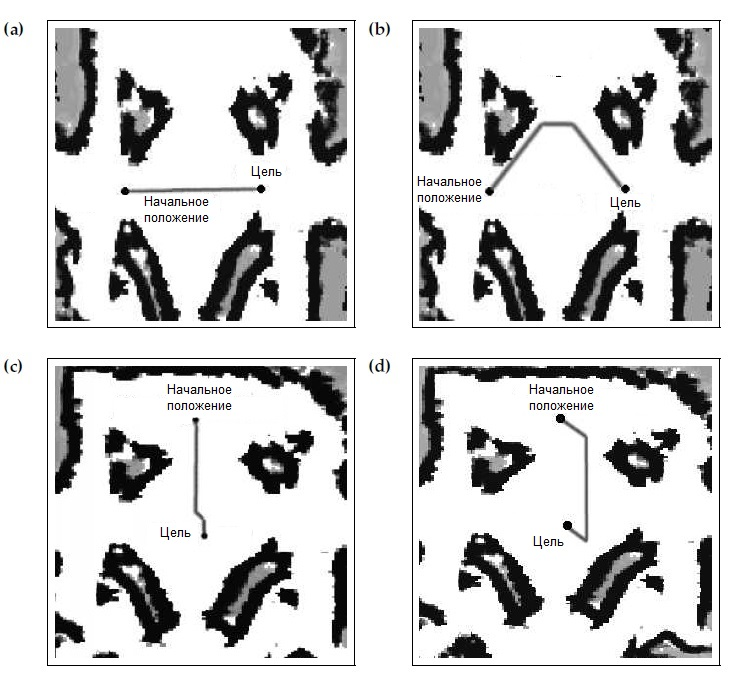
\includegraphics[width=1\linewidth]{161orig}}
	\caption{ ( Рис. 16.1 Примеры пути робота в большой, открытой среде для двух разных конфигураций (верхний и нижний ряд). На схемах (a) и (c) показаны пути, сгенерированные обычным динамическим программирующим планировщиком пути, игнорирующем неопределённость восприятия робота. Схемы (b) и (d) получены с использованием дополненного MDP планировщика, который учитывает неопределённость и избегает области, где робот имеет большую вероятность заблудиться. Собственность Николаса Роя, МИТ ( Nicholas Roy, MIT).) }
	\label{fig:161orig}
\end{figure}

\begin{figure}[H]
	\center{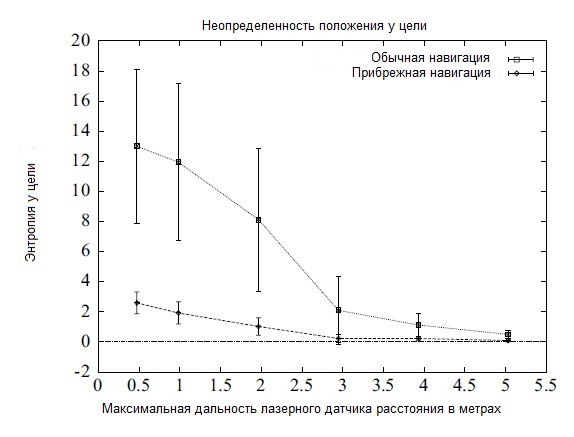
\includegraphics[width=0.85\linewidth]{162orig}}
	\caption{ ( Рис. 16.2 Сравнение эффективности планирования MDP и дополненного планирования MDP. Здесь показана неопределённость (энтропия) целевого местоположения как функции дальности согласно показаниям датчика. Собственность Николаса Роя, МИТ (Nicholas Roy, MIT).) }
	\label{fig:162orig}
\end{figure}

\textbf{16.3.4	Применение в навигации мобильного робота}\\

Алгоритм AMDP весьма практичен. В контексте навигации мобильного робота AMDP позволяет роботу учитывать общий уровень «замешательства» при выборе действий. Это относится не только к текущей мгновенной неопределённости, но и к будущей ожидаемой неопределённости, с которой робот может столкнуться при выборе действий.

Рассматриваемый пример включает навигацию робота в известной среде и уже приводился во вводной части книги, на Рис. 1.2 на странице 7 ???. Очевидно, уровень «замешательства» зависит от того, где именно выполняется навигация. Робот проходит через большую зону, лишённую признаков, и постепенно утрачивает информацию о том, где именно он находится. Это отражено условной вероятностью $p(\bar{b}' | u, \bar{b})$, которая в таких зонах с высоким правдоподобием увеличивает энтропию гипотезы. В зонах с признаками, пригодными для локализации, то есть вблизи стен с различимыми признаками, неопределённость, скорее всего, уменьшится. AMDP обрабатывает такие ситуации и генерирует политики, минимизирующие время прибытия, с одновременной максимизацией определённости в момент прибытия к целевому местоположению. Поскольку неопределённость является оценкой ошибки по отношению к настоящему местоположению, она является хорошей мерой шансов того, что робот действительно прибудет к требуемой локации. 

\begin{figure}[H]
	\center{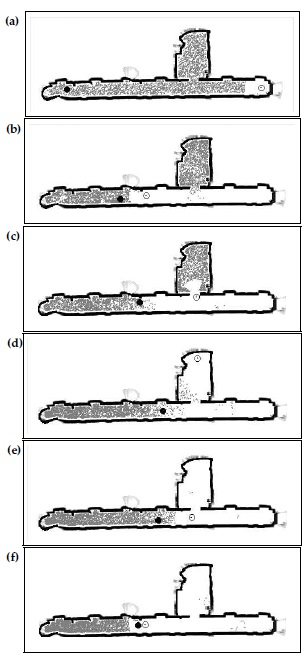
\includegraphics[width=0.65\linewidth]{163orig}}
	\caption{ ( Рис. 16.3 Политика, вычисленная с помощью расширенной версии AMDP с обученным представлением состояния. Заданием является обнаружение нарушителя. Серые частицы извлекаются из распределения возможных местоположений человека, вначале равномерно распределенных по (a). Чёрная точка - истинное (ненаблюдаемое) положение человека. Открытый круг – наблюдаемое положение робота. Эта политика успешно работает  с высокими значениями правдоподобия. Собственность Николаса Роя, МИТ и Джеффри Гордона, СМУ ( Nicholas Roy, MIT and Geoffrey Gordon, CMU). ) }
	\label{fig:163orig}
\end{figure}

На Рис. 16.1 показаны примеры траекторий для двух групп (сочетаний начальных и конечных местоположений). Схемы слева соответствуют планировщику MDP, который не учитывает неопределённость робота. Дополненный планировщик MDP генерирует траектории наподобие показанных на фото. На Рис. 16.1a и b, от робота требуется продвинуться через большое открытое пространство, примерно 40 метров шириной. Алгоритм MDP, не учитывая возросший риск заблудиться на открытом пространстве, генерирует политику кратчайшего пути от точки старта до целевой локации. Планировщик AMDP, напротив, генерирует политику передвижения вблизи препятствий, где у робота есть большая вероятность получить информативные измерения датчиков ценой возросшего времени передвижения. Аналогично, на Рис. 16.1c и d показана ситуация, где целевая локация близка к центру открытой области без признаков. Здесь планировщик AMDP распознает, что проход около знакомых объектов уменьшает неопределённость положения, успешно увеличивая шансы достижения целевой локации.

На Рис. 16.2 показано сравнение эффективности между стратегией навигации AMDP и подходом MDP. В частности, показана энтропия гипотезы робота в целевой локации, как функции характеристик датчика. На этом графике варьируется максимальное расстояние восприятия для изучения воздействия ухудшения датчиков. Как показано на графе, у AMDP существенно более высокие шансы успеха и разница наиболее велика для плохих датчиков. Для датчиков с большой дальностью действия разница постепенно исчезает. Это неудивительно, поскольку при наличии хороших датчиков количество информации, которая может быть получена, меньше зависит от конкретного положения робота.\\

ПРИБРЕЖНАЯ НАВИГАЦИЯ\\

Способность учитывать неопределённость и избегать её привела к созданию так называемой \textit{прибрежной навигации} в алгоритмах использования AMDP для навигации робота. Название указывает на схожесть с кораблями, которые, до изобретения спутниковой навигации, часто оставались вблизи береговой линии, чтобы не потерять возможность отслеживать своё местоположение.

Завершим обсуждение AMDP замечанием, что выбор статистики $f$ в некоторой степени, произволен. Признаки могут добавляться по необходимости, но это вызывает ожидаемый рост вычислительной сложности. Современные исследования позволили создать алгоритмы, которые обучаются статистикам $f$, используя нелинейные методы уменьшения размерности. На Рис. 16.3 показан результат такого обучающегося алгоритма, применяемого к задаче поиска движущегося нарушителя в здании. Здесь обучающийся алгоритм идентифицирует шестимерное представление состояния, отражающее гипотезу робота для любой применимой стратегии преследования. Серые частицы представляют собой гипотезы робота относительно местонахождения нарушителя. Как показано в этом примере, AMDP с обучением выражению состояния успешно генерирует довольно сложную стратегию: сначала робот осматривает часть коридора, оставаясь достаточно близко от комнаты, чтобы нарушитель не мог покинуть ее. Затем робот осматривает комнату за достаточно короткое время, чтобы нарушитель не сумел пройти по коридору незамеченным. Наконец, после осмотра комнаты, робот продолжает преследование по коридору.\\

\textbf{16.4	Monte Carlo POMDP}\\

\textbf{16.4.1	Использование наборов частиц}\\

Последний алгоритм, обсуждаемый в этой главе, это решение многочастичного фильтра для POMDP, называемое MC-POMDP, сокращение от "Monte Carlo POMDP". MC-POMDP находит функцию дохода, определённую наборами частиц. Пусть $\mathcal{X}$ будет набором частиц, выражающим гипотезу $b$. Тогда функция дохода может выражаться в следующем виде\\

(16.10)
$$V\,:\,\mathcal{X}\longrightarrow \Re$$

Это выражение имеет ряд преимуществ, но создаёт и затруднения. Ключевым преимуществом является возможность выражения функций ценности по произвольным пространствам состояний. Фактически, среди всех алгоритмов, которые обсуждались до сих пор, MC-POMDP – единственный, в котором не требуется конечное пространство состояний. Далее, в MC-POMDP для отслеживания гипотез используются многочастичные фильтры. Мы уже видели несколько примеров применения многочастичных фильтров. MC-POMDP расширяет использование многочастичных фильтров для задач планирования и управления.

Основная трудность использования наборов частиц в POMDP состоит в выражении функции дохода. Пространство всех наборов частиц любого данного размера $M$ имеет размерность $M$. Более того, вероятность того, что какой-либо из наборов частиц будет наблюдаться дважды, равна нулю в силу стохастической природы генерации частиц. В результате, необходимо выражение для $V$, которое можно обновлять с помощью некоторого набора частиц, но затем представить значение для другого набора частиц, который алгоритм MC-POMDP ещё никогда не встречал. Другими словами, требуется \textit{обучающийся алгоритм}. MC-POMDP использует алгоритм \textit{ближайшего соседа}, используя локально взвешенную интерполяцию при интерполяции между разными гипотезами.\\

\textbf{16.4.2	Алгоритм MC-POMDP} \\

В Таблице 16.3 приводится базовый алгоритм MC-POMDP с использованием нескольких вложенных циклов.  Самый внутренний цикл, в строках с  6 по 16 в Таблице 16.3, обновляет функцию дохода $V$ для конкретной гипотезы $\mathcal{X}$. Это делается моделированием набора возможных последующих гипотез для каждого применимого действия управления $u$. Это моделирование выполняется в строках с 9 по 12. После этого собирается значение локального дохода для каждого из применимых действий (строка 13). Обновление функции дохода происходит в строке 16, где $V$ просто устанавливается в значение, максимальное для всех $Q_u$.\\

\begin{table}[H]
\begin{center}
\begin{tabular}{|l|}
\hline
{}\\
1:\textbf{ Algorithm MC-POMDP}$(b_0,V):$\\
2:\hspace{5mm}$\textit{поаторять до сходимости}$\\
3:\hspace{10mm}$\textit{выборка}\,x\sim b(x)\qquad\qquad\qquad\qquad//\text{ инициализация}$\\
4:\hspace{10mm}$\textit{инициализировать}\,\mathcal{X}\,\textit{with}\,M\,\textit{выборки из}\,b(x)$\\
5:\hspace{10mm}$\textit{повторять до конца эпизода}$\\
6:\hspace{15mm}$\textit{для всех действий управления u выполнить}\qquad//\text{функция обновления дохода}$\\
7:\hspace{20mm}$Q(u)=0$\\
8:\hspace{20mm}$\textit{повторить n раз}$\\
9:\hspace{25mm}$\textit{выбрать случайный}\,x\in\mathcal{X}$\\
10:\hspace{24mm}$\textit{выборка}\,x'\sim p(x'|u,x)$\\
11:\hspace{24mm}$\textit{выборка}\,z\sim p(z|x')$\\
12:\hspace{24mm}$\mathcal{X}'=\textbf{Particle\_filter}\,(\mathcal{X},u,z)$\\
13:\hspace{24mm}$Q(u)=Q(u)+\frac{1}{n}\gamma[r(x,u)+V(\mathcal{X}')]$\\
14:\hspace{20mm}$\textit{endrepeat}$\\
15:\hspace{15mm}$\textit{endfor}$\\
16:\hspace{15mm}$V(\mathcal{X})=\underset{u}{\max}\,Q(u)\qquad\qquad//\text{функция обновления дохода}$\\
17:\hspace{15mm}$u^*=\underset{u}{\text{argmax}}\,Q(u)\qquad\qquad//\text{выбор жадного действия}$\\
18:\hspace{15mm}$\textit{выборка}\,x'\sim p(x'|u,x)\qquad//\text{моделирование перехода состояния}$\\
19:\hspace{15mm}$\textit{выборка}\,z\sim p(z|x')$\\
20:\hspace{15mm}$\mathcal{X}'=\textbf{Particle\_filter}\,(\mathcal{X},u,z)\,\,\,//\text{вычислить новую гипотезу}$\\
21:\hspace{15mm}$\textit{установить}\,x=x';\mathcal{X}=\mathcal{X}'\qquad\qquad//\text{обновление состояния и гипотезы}$\\
22:\hspace{10mm}$\textit{endrepeat}$\\
23:\hspace{5mm}$\textit{endrepeat}$\\
24:\hspace{5mm}$\textit{return}\,\,V$\\
{}\\
\hline
\end{tabular}
\caption{(Таблица 16.3    Алгоритм MC-POMDP.)}
\end{center}
\end{table}

После этого выполняется локальный обратный проход в котором MC-POMDP моделирует физическую систему для генерации нового набора частиц $\mathcal{X}$ . Это моделирование выполняется в строках с 17 по 21. В нашем примере при обновлении всегда выбирается жадное действие (строка 17), однако, на практике может оказаться выигрышнее выполнение случайного действия. С помощью перехода к новой гипотезе $\mathcal{X}$, в итерационном алгоритме MC-POMDP выполняется обновление на другую гипотезу состояния. Выполняя итерации для целых эпизодов (внешние циклы в строках со 2 по 5), функция дохода постепенно обновляется везде.

Ключевой открытый вопрос касается выражения функции $V$. MC-POMDP использует локальный обучающийся алгоритм, напоминающий алгоритм ближайших соседей. В нём конструируется набор эталонных гипотез $\mathcal{X}_i$ со связанными значениями $V_i$. При появлении запроса с прежде невидимым набором частиц $\mathcal{X}_{\text{query}}$, MC-POMDP идентифицирует $K$ «ближайший» набор частиц в памяти. Определение подходящей концепции близости для наборов частиц требует дополнительных допущений. В оригинальной реализации, MC-POMDP сворачивает каждую частицу гауссовой функцией с малой, фиксированной ковариацией, a затем вычисляет KL-дивергенцию между результирующими смесями гауссиан. В двух словах, этот шаг даст возможность определить $K$ ближайших эталонных наборов частиц $\mathcal{X}_1,..., \mathcal{X}_K$, с соответствующими мерами расстояния, обозначаемыми $d_1,..., d_K$ (заметим, что KL- дивергенция, технически, говоря, не расстояние, поскольку она ассиметрична). Ценность запроса набора частиц $\mathcal{X}_{\text{query}}$, получается согласно следующей формуле\\

(16.11)
$$V(\mathcal{X}_{\text{query}})=\eta\sum_{k=1}^K\frac{1}{d_k}V_k$$

где $\eta=[\varSigma_k\frac{1}{d_k}]^{-1}$.   Здесь $\mathcal{X}_k$   это $k$-ая эталонная гипотеза в наборе $K$
ближайших соседей, и $d_k$ –соответствующая дистанция до запрашиваемого набора.\\

МЕТОД ИНТЕРПОЛЯЦИИ ШЕПАРДА \\
Эта формула интерполяции, известная как \textit{метод интерполяции Шепарда}, объясняет, как вычислить
$V(\mathcal{X}')$ в строке 13 Таблицы 16.3.

Обновление в строке 16 включает неявную дифференциацию. Если эталонный набор уже содержит $K$ наборов частиц, расстояние меньше определяемого пользователем порога, соответствующие $V$ -значения обновляются просто пропорционально их вкладу в интерполяцию:\\

(16.12)
$$V_k\longleftarrow V_k+\alpha\,\eta
\,\frac{1}{d_k}(\underset{u}{\max}Q(u)-V_k)$$

где $\alpha$ – скорость обучения.  Выражение $max_u  Q(u)$ является «целевым» значением для функции $V$, а $\eta
\,\frac{1}{d_k}$ вклад k-й эталонной частицы набора в методе интерполяции Шепарда.

Если имеется меньше, чем $K$ наборов частиц, расстояние которых падает ниже порогового значения, запрашиваемый набор частиц просто добавляется к эталонному, с ассоциированным значением $V = max_u Q(u)$. Таким образом, набор эталонных наборов частиц растёт со временем. Значение $K$ и определяемый пользователем порог расстояния определяет гладкость функции ценности MC-POMDP. На практике, выбор соответствующих значений потребует некоторого осмысления, поскольку очень легко превысить объем памяти обычного персонального компьютера эталонным набором, если выбрать порог слишком плотно.\\

\textbf{16.4.3	Математический вывод MC-POMDP}\\

Алгоритм MC-POMDP основан на нескольких аппроксимациях: использование наборов частиц образует первое приближение. Вторая – это использование локального алгоритма обучения для выражения $V$, которое исключительно приближенное. Третья аппроксимация - использование обратного прохода по методу Монте-Карло функции ценности. Каждая из этих аппроксимаций ставит под угрозу сходимость базового алгоритма.

Математическая обоснованность использования многочастичных фильтров была уже описана в Главе 4. Шаг обновления по методу Монте-Карло следует из общего уравнения обновления POMDP (15.43) на странице 532 ???, и повторно приводится ниже:\\

(16.13)
$$V_T(b)=\gamma\,\underset{u}{\max}\left[ r(b,u)+\int V_{T-1}(B(b,u,z))p(z|u,b)dz\right] $$

Аппроксимация по методу Монте-Карло выводится полностью аналогично выводу AMDP. Начнём с вероятности измерения $p(z | u, b)$, которая разрешается следующим образом:\\

(16.14)
$$p(z|u,b)=\iint p(z|x')p(x'|u,x)b(x)dx\,dx'$$

Похожим образом, получаем для $r(b, u)$:\\

(16.15) 
$$r(b,u)=\int r(x,u)b(x)dx$$

Это позволяет переписать (16.13) следующим образом:\\

(16.16)
\begin{equation*}
\begin{split}
V_T(b)&=\gamma\,\underset{u}{\max}[ \int r(x,u)b(x)dx\\
&\hspace{5mm}+\int V_{T-1}(B(b,u,z))[ \iint p(z|x')p(x'|u,x)b(x)dx\,dx'] dz] \\
&=\gamma\,\underset{u}{\max}\iiint[r(x,u)+V_{T-1}(B(b,u,z))p(z|x')p(x'|u,x)]b(x)dx\,dx'\,dz
\end{split}
\end{equation*}

Аппроксимация по методу Монте-Карло для этого интеграла сейчас представляет алгоритм выборки с несколькими переменными, что требует выполнения выборки $x\sim b(x), x'\sim p(x' | u, x)$ и $z\sim p(z|x')$.  Как только мы получим $x, x'$, и $z$, станет возможно вычислить $B(b, u, z)$ с помощью байесовского фильтра. Затем вычислим $V_{T-1}(B(b, u, z))$, используя локальный обучающийся алгоритм, а $r(x, u)$ – простым поиском. Заметим, что все эти шаги реализованы в строках с 7 по 14 Таблицы 16.3, а финальная максимизация выполняется в строке 16.

Локальный обучающийся алгоритм, который играет центральную роль в MC- POMDP, может легко нарушить любую сходимость алгоритма Монте-Карло. Не будем пытаться охарактеризовать условия, при которых локальное обучение может дать точную аппроксимацию, а, вместо этого, просто отметим необходимость соблюдения осторожности при установке различных параметров.\\

\textbf{16.4.4	Практические соображения}\\

Из трёх приближений POMDP, приведённых в этой главе, MC- POMDP разработано хуже всех и, потенциально, наименее эффективно. Его аппроксимация основана на обучающимся алгоритме для выражения функции дохода. Реализация алгоритма MC-POMDP может быть весьма затруднена. Требуется хорошее понимание гладкости функции ценности, а также, количества частиц, которое будет использоваться.

Оригинальная реализация алгоритма MC-POMDP даёт результат, показанный на Рис. 16.4. Робот, показанный на Рис. 16.4a, находится около объекта, который можно взять, и который можно обнаружить с помощью камеры. Однако, изначально объект расположен вне поля восприятия робота. Успешная политика, таким образом, будет включать три этапа. Этап поиска, во время которого робот поворачивается, пока не обнаружит объект, этап движения, во время которого робот центрует своё положение относительно объекта так, чтобы его можно было захватить, и финальное действие захвата. Комбинация активного восприятия и поведения, нацеленного на достижение цели превращают это в относительно сложную вероятностную проблему управления.

На Рис. 16.4b показаны несколько примерных эпизодов, в которых робот успешно поворачивался, двигался и хватал объект. Показанные траектории проектируют движение в 2D. Численные результаты приведены на Рис. 16.4c, где показан коэффициент успешности как функция обновления итерационного алгоритма MC-POMDP. 4000 итераций обратного прохода параметра дохода потребовали примерно 2 часа вычислительного времени на маломощном персональном компьютере, а средняя эффективность алгоритма находится на уровне 80\%. Оставшиеся 20\% неудачных попыток относятся, в основном, к конфигурациям, в которых робот оказался неспособен определить своё положение для захвата объекта. Отчасти, это стало следствием множества аппроксимаций в MC-POMDP. 

\begin{figure}[H]
	\center{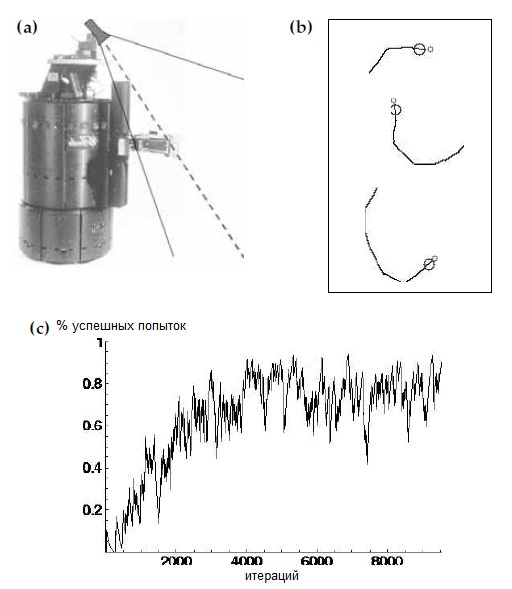
\includegraphics[width=0.8\linewidth]{164orig}}
	\caption{ ( Рис. 16.4 Задание робота «найти и взять»: Мобильный робот с захватом и камерой, держащий целевой предмет(a).  Представление на плоскости трёх успешных выполнений политики, в которых робот вращался, пока не увидит объект, а затем захватывал его(b). Коэффициент успешности, как функция количества шагов планирования, оценённая моделированием.(c)) }
	\label{fig:164orig}
\end{figure}

\textbf{16.5	Выводы}\\

В этом разделе было представлено три приближенных вероятностных алгоритма планирования и управления, с различными показателями практической применимости. Все три алгоритма основаны на аппроксимации функции ценности POMDP, но различаются способом этой аппроксимации.\\

•	Аппарат QMDP учитывает неопределённость только для одного выбора действия. Он основан на допущении, что после следующего действия управления, состояние среды внезапно становится наблюдаемым. Полная наблюдаемость делает возможным применение MDP-оптимальной функции дохода. QMDP обобщает функцию ценности MDP в пространства гипотез с помощью оператора математического ожидания. В результате, планирование в QMDP отличается от такового в MDP, но функция дохода, в общем, переоценивает настоящее значение гипотезы состояния.\\

•	Обобщения алгоритма QMDP объединяют MDP-оптимальную функцию дохода с последовательностью обратных проходов POMDP.  При комбинировании с $T$ \textit{шагами обратных проходов} POMDP, результирующая политика подразумевает действия сбора информации с горизонтом $T$, а затем полагается на допущение QMDP о полной наблюдаемости состояния. Чем больше горизонт $T$, тем ближе результирующая политика к полному решению POMDP.\\

•	Алгоритм AMDP использует другую аппроксимацию. Он проецирует гипотезу в отображение более низкой размерности, по которой затем выполняется точный итерационный алгоритм. «Классическое» выражение состоит из наиболее вероятного состояния гипотезы, и энтропией гипотезы. В этом выражении, AMDP работают так же, как MDP с одним добавленным измерением в представлении состояния, измеряющим глобальное состояние неопределённости робота.\\

•	Для реализации AMDP становится необходимым \textit{обучить} переход состояний и функцию награды в пространстве гипотез низкой размерности. AMDP достигает этого в течение первой фазы, в которой статистики кэшируются в таблицы с возможностью поиска, выражая переход состояний и функцию дохода. Поэтому, AMDP работает по обученной модели, и обладает точностью, определяемой её точностью.\\

•	Применение AMDP в навигации в известных средах называется \textit{прибрежной навигацией}. В этом методе навигации учитывается неопределённость,  и движение подбирается так, чтобы найти компромисс между  общей длиной пути и неопределённости, накопленной вдоль траектории. Результирующие траектории существенно отличаются от решений без использования вероятности. Робот, выполняющий «прибрежную навигацию» избегает областей, в которых шансы заблудиться велики. Временная потеря ориентации допустима, если позже робот способен выполнить повторную локализацию с высокой вероятностью.\\

•	Алгоритм MC-POMDP это версия POMDP с использованием многочастичного фильтра. В нем вычисляется функция дохода, определённая по наборам частиц. Для реализации такой функции дохода MC-POMDP необходимо использовать локальный обучающийся метод, использующий локальное взвешенное правило обучения в комбинации с проверкой на близость на основе KL-дивергенции. В MC-POMDP затем используется выборка методом Монте-Карло для реализации приблизительного обратного прохода итерационного алгоритма. Результирующий алгоритм представляет собой полноценный алгоритм POMDP, вычислительная точность и сложность которого являются функциями параметров обучающегося алгоритма.\\

Ключевой урок, который можно вынести из этой главы, состоит в том, что существует несколько аппроксимаций, вычислительная сложность которых очень близка к MDP, но которые все ещё учитывают неопределённость состояния. Неважно, насколько груба аппроксимация, алгоритмы, которые учитывают неопределённость состояния, обычно существенно более надёжны по сравнению с алгоритмами, которые полностью ее игнорируют. Даже один новый элемент в векторе состояний, который измеряет глобальную неопределённость в одномерном виде, может создать огромную разницу в производительности робота.\\

\textbf{16.6	Библиографические примечания}\\

Литература по решению приближенной задачи POMDP подробно обсуждалась в предыдущей главе (15.7). Алгоритм QMDP, описанный в этой главе, принадлежит Литтману (Littman et al., 1995). Алгоритм AMDP для выражения фиксированного дополненного состояния был разработан Роем (Roy et al., 1999). Позже, Рой (Roy et al., 2004) обобщил его до выражения обученного состояния. Трун (Thrun, 2000a) вывел алгоритм Монте-Карло POMDP.\\

\textbf{16.7	Упражнения}\\

1.	В этом вопросе, требуется разработать AMDP, решающий простую задачу навигации. Рассмотрим следующую среду с 12 дискретными состояниями.

\begin{figure}[H]
	\center{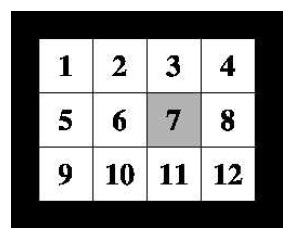
\includegraphics[width=0.5\linewidth]{16sreda}}
	\label{fig:16sreda}
\end{figure}

Вначале, робот помещён в некоторое случайное местоположение, равномерно выбранных из 12 состояний. Целью является достижение состояния 7. В любой момент времени робот перемещается на север, восток, запад или юг. Его единственный датчик - это бампер: при столкновении с препятствием, бампер срабатывает, и робот не меняет состояние. Робот не может воспринимать состояние, в котором находится, и не может определить, с какой стороны сработал бампер. В этой задаче нет шума и неопределённости начального положения (распределение будем считать равномерными).\\

(a)	Какое минимальное количество состояний необходимо иметь AMDP? Описать все.\\

(b)	Сколько из этих состояний достижимы из начального состояния AMDP? Описать все.\\

(c)	Сейчас допустим, что робот начинает в состоянии 2 (которого он не знает, поэтому его внутренняя гипотеза другая). Нарисовать схему перехода между всеми состояниями AMDP, которые можно достичь за четыре действия.\\

(d)	Для этого типа задачи (датчики и движение робота без шума, конечные пространства состояний, действий, измерений), можно ли придумать более компактное выражение по сравнению с AMDP, которого все ещё будет достаточным для нахождения оптимального решения?\\

(e)	Для этого типа задачи (датчики и движение робота без шума, конечные пространства состояний, действий, измерений), можно ли сконструировать пространство состояний, для которого AMDP окажется неспособен найти оптимальное решение?\\

2.	В предыдущей главе, мы узнали о \textit{задаче тигра} (Упражнение 1 на странице 544 ???). Какие изменения этой задачи позволят QMDP найти оптимальное решение? Подсказка: Возможных ответов несколько.\\

3.	В этом упражнении требуется определить \textit{размер} пространства гипотез состояний. Используем следующую таблицу:\\
{}\\
\begin{tabular}{c|c|l|l|l}
Номер &Количество &датчики&Переход&Начальное   \\
задачи&состояний&{}&состояний&состояние\\
\hline
\#1&3&совершенный&без шума&известно\\ \hline
\#2&3&совершенный&зашумленный&известно\\
\hline
\#3&3&без шума&без шума&неизвестно\\
{}&{}&{}&{}& (равномерное)\\
\hline
\#4&3&зашумленный&без шума&известно\\
\hline
\#5&3&зашумленный&без шума&неизвестно\\
{}&{}&{}&{}& (равномерное)\\
\hline
\#6&3&нет&без шума&неизвестно\\
{}&{}&{}&{}& (равномерное)\\
\hline
\#7&3&нет&зашумленный&известно\\
\hline
\#8&1-мерное &совершенный&зашумленный&известно\\
{}&непрерывное&{}&{}& {}\\
\hline
\#9&1-мерное &зашумленный&зашумленный&известно\\
{}&непрерывное&{}&{}& {}\\
\hline
\#10&2-мерное &зашумленный&зашумленный&неизвестно\\
{}&непрерывное&{}&{}& (равномерное)\\
\hline
\end{tabular}\\

Совершенный датчик всегда даёт полную информацию о состоянии. Датчик без шума может предоставлять частичную информацию о состоянии, но делает это без элемента случайности. Зашумлённый датчик может не только давать частичную информацию, но и подвержен помехам. Переход состояний без шума детерминирован, а стохастический переход состояний оказывается зашумлённым. Наконец, будем различать только два типа начальных условий, в одном из которых начальное состояние известно с абсолютной уверенностью, а в другом – совершенно неизвестно и априорное распределение однородно.\\

Вопрос: Каков размер достижимого состояния гипотез для всех 10 задач?\\ Подсказка: Он может быть конечным или бесконечным, в бесконечном случае указать размерность пространства гипотез.\\

4.	Требуется поразмышлять о критических режимах планировщика AMDP. В частности, AMDP \textit{изучает} переход состояний и функции дохода. Поразмышлять о том, что может нарушить работу такой обученной модели, использующей итерационный алгоритм. Указать, по меньшей мере, три вида проблем, и детально их обсудить.\\

 
\end{document}